\iffalse
\begin{frame}
	\frametitle{Médical : exemple de la grippe}
	\begin{center}
		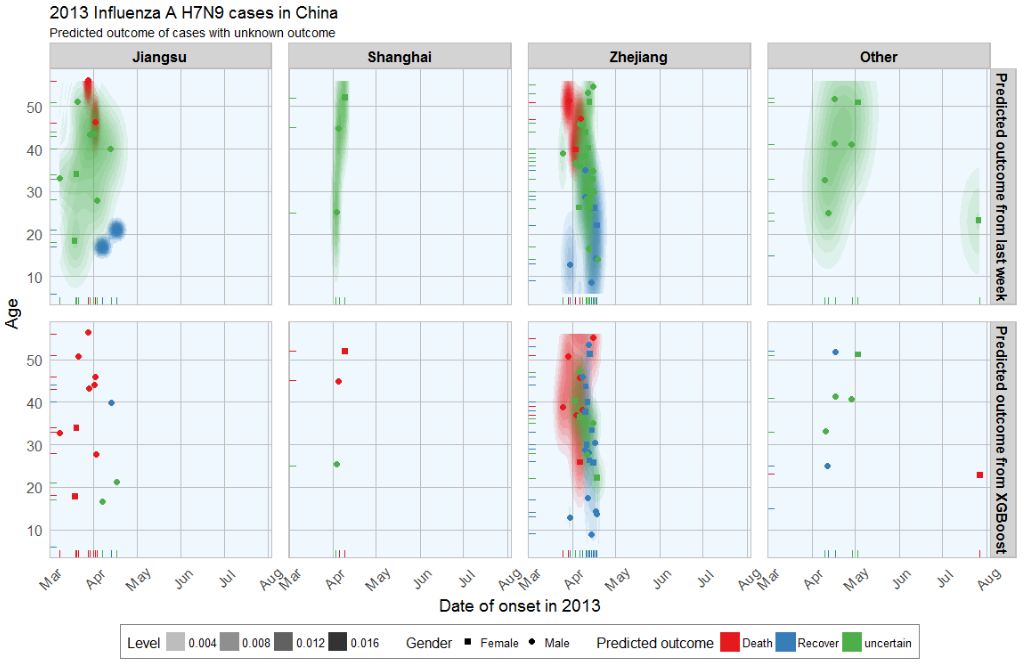
\includegraphics[width=.8\textwidth]{images/utilisation/flue}
	\end{center}
	\rule{0pt}{0pt}\hfill{\fontsize{.15cm}{0cm}\selectfont{\textit{Source : \texttt{https://shiring.github.io/machine\_learning/2016/12/02/flu\_outcome\_ML\_2\_post}}}}
\end{frame}
\fi

\begin{frame}
	\frametitle{Challenges Kaggle}
	\onslide<1->{
		\begin{center}
			\textit{En 2015 sur Kaggle, 17 solutions gagnantes sur 29 utilisaient XGBoost.}
		\end{center}
	}%
	\onslide<2>{
		\begin{itemize}
			\itemperso{1\up{er}}Knowledge Discovery and Data Mining Cup 2016 (V. Sandulescu).
			\itemperso{1\up{er} et 3\up{ème}}CERN LHCb experiment Flavour of Physics competition 2015 (V. Mironov).
			\itemperso{1\up{er}}Caterpillar Tube Pricing competition (M. Filho).
			\itemperso{2\up{ème}}Airbnb New User Bookings (K. Kuroyanagi).
			\itemperso{2\up{ème}}Allstate Claims Severity (A. Noskov).
			\itemperso{10\%}Higgs Boson Competition (T. Chen).
			\itemperso{...}
		\end{itemize}
	}
\end{frame}

\begin{frame}
	\frametitle{Un exemple concret}
	\begin{center}
		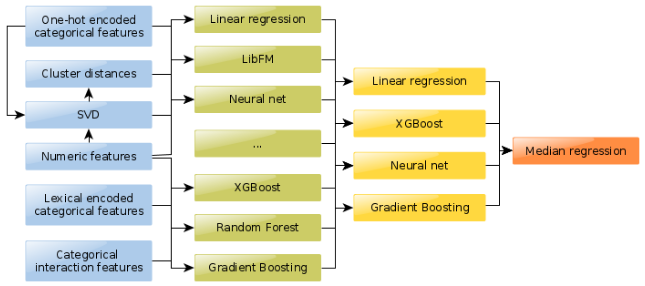
\includegraphics[width=.9\textwidth]{images/utilisation/pipeline}
	\end{center}
	\rule{0pt}{0pt}\hfill{\fontsize{.15cm}{0cm}\selectfont{\textit{Source : \texttt{http://blog.kaggle.com/2017/02/27/allstate-claims-severity-competition-2nd-place-winners-interview-alexey-noskov/}}}}
\end{frame}

\begin{frame}
	\frametitle{En entreprise}
	\textit{Des données difficiles à obtenir...}\vspace*{.2cm}
	\begin{itemize}
		\itemperso{}ODPS Cloud Service (Alibaba)\vspace*{.2cm}
		\itemperso{}Tencent (QQ)\vspace*{.2cm}
		\itemperso{}AutoHome\vspace*{.2cm}
		\itemperso{}AXA, Expedia, Amazon,...\vspace*{.2cm}
	\end{itemize}
\end{frame}